\section{melcomp\_3}

At the Visual Neuroscience Summer School I spoke with Laurence Maloney about this work, and about his own work on colour constancy \citep{maloney_computational_1984,maloney_color_1986}, and he suggested that I consider a simple game: given cone catches from an unknown surface under an unknown illuminant, guess the illuminant. If you are able to guess the illuminant with a moderate accuracy, you've cracked colour constancy.

Whilst this had been an implicit thread throughout much of the work to this point, it was a neat idea to be spelled out so clearly. I had my reservations - from my experience with the rotational corrective transform (Figure \ref{fig:viewpoint}) I had seen that a correction (to an illuminant-independent space) seemed possible even without explicit knowledge of the illuminant. Of course one could get an estimate of the illuminant from such a computation, but it was a potential output, not a requisite input. All the same, I thought it would be a relatively neat and simple thing to show.

In melcomp\_3 I attempt this, using the framework of linear modelling which Laurence is so well known for. It is used in a relatively rudimentary way here, compared to the complex manner in which Laurence uses it in his thesis \citep{maloney_computational_1984}. Whereas there he uses it to compute a solution to colour constancy, here I only use it to define my light sources, and then query which signals can predict the light sources so defined.

I start in much the same way as I have done in melcomp\_1 and 2, by loading data upon which to perform the computations. This time, I used an extended subset of the \citet{vrhel_measurement_1994} dataset, considering anything which could be considered natural rather than the small selection previously needed, on the basis that to consider correlation I would need an increased number of datapoints. At this stage I was using the \gls{SP} fundamentals, mainly in order to obey the rules of the traditional \gls{MB} diagram \citep{macleod_chromaticity_1979}. Again I used the Granada data \citep{hernandez-andres_color_2001}. From these inputs, I compute the $[L,M,S,R,I]$ values, and the corresponding \gls{MB} chromaticity values and pseudo-MB values ($i_{\text{MB}}$ and $r_{\text{MB}}$) for each surface under each illuminant.

I also compute the principal component representation of each illuminant. A variable weighting was specified, which gave most importance to wavelengths between the peak sensitivity of the S-cones and the peak sensitivity of the L-cones, before tailing off at each end (shown in Figure \ref{fig:VW}). This weighting is an important and difficult choice, and no entirely sensible solution is forthcoming\footnote{Do we care more about certain wavelengths than others? Yes. Which ones and by how much by? Unknown, and evolutionarily circular.}. \citet{maloney_evaluation_1986} discusses this further. %read and say more

% \begin{figure}[htbp]
%  \includegraphics[max width=\textwidth]{figs/comp/melcomp_3/?.png}
%  \caption{The variable weightings applied during the \gls{PCA} analysis. Generated by tracing the upward ramp of the S-cone sensitivity being used, plateauing at unity until the decrease of the L-cone sensitivity, and then following the decrease of the L-cone sensitivity.}
%  \label{fig:VW}
% \end{figure} 

The principal components identified are shown in Figure \ref{fig:PCA}. The first three components account for X,Y, and Z\% of variance respectively.

\begin{figure}[htbp]
 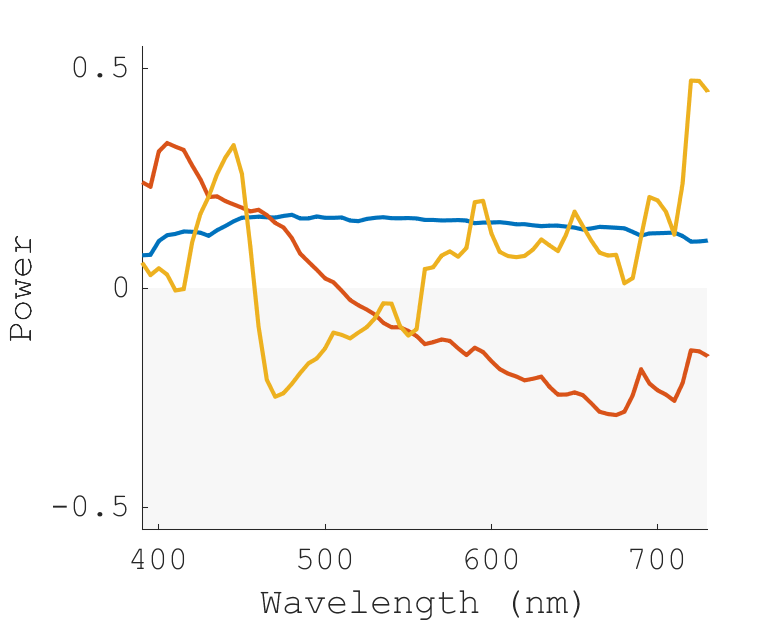
\includegraphics[max width=\textwidth]{figs/comp/melcomp_3/8.png}
 \caption{The first 3 principal components for the Granada daylight dataset, conditional on the variable weighting shown in Figure \ref{fig:PCA}.}
 \label{fig:VW}
\end{figure} 

% Might be neat to show the chromatic effect of each of these PCs?

I then computed the correlation between a large number of candidate signals and the scores for different components of the \glspl{SPD}. This is shown in \ref{fig:19}. Plain talk: which signal was best at predicting each element of the daylight spectra upon a scene?

\begin{figure}[htbp]
 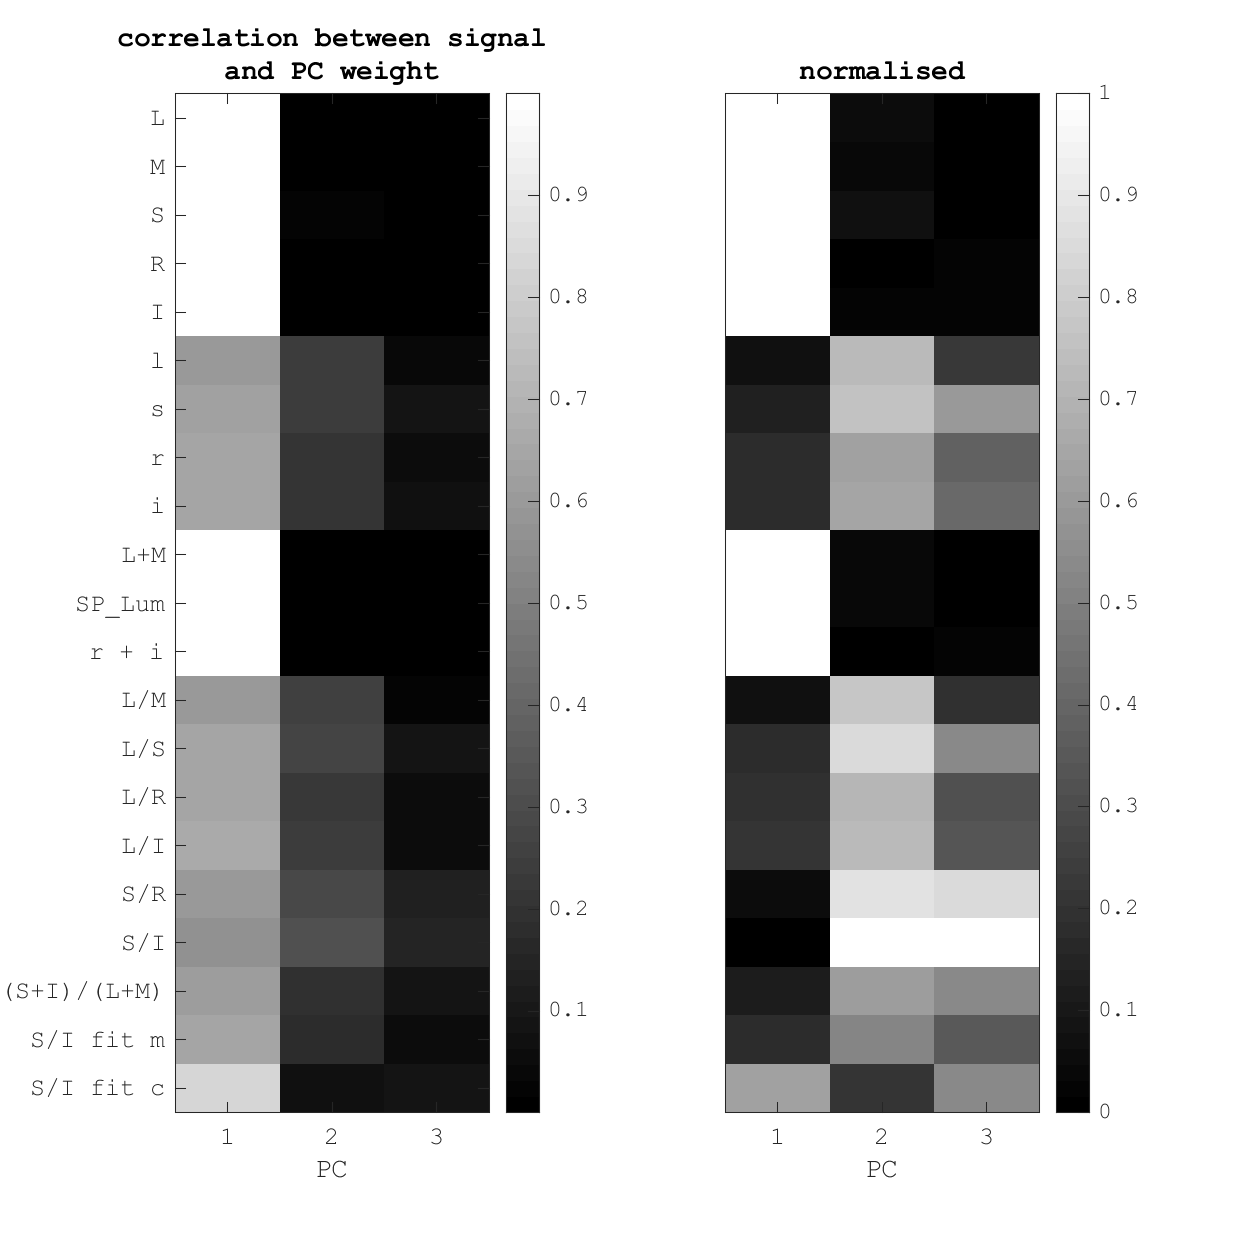
\includegraphics[max width=\textwidth]{figs/comp/melcomp_3/19.png}
 \caption{\hl{Caption}}
 \label{fig:19}
\end{figure} 

\begin{figure}[htbp]
 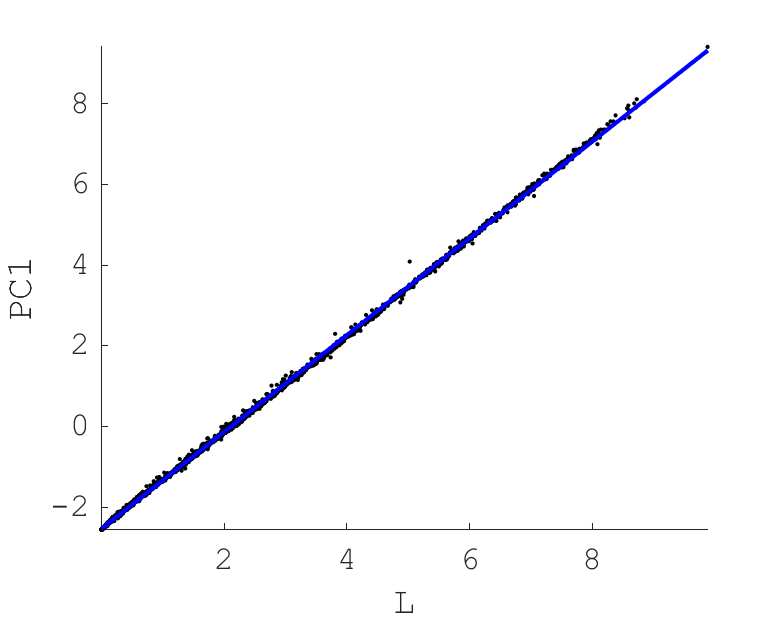
\includegraphics[max width=\textwidth]{figs/comp/melcomp_3/20.png}
 \caption{\hl{Caption}}
 \label{fig:L-PC1}
\end{figure} 

\begin{figure}[htbp]
 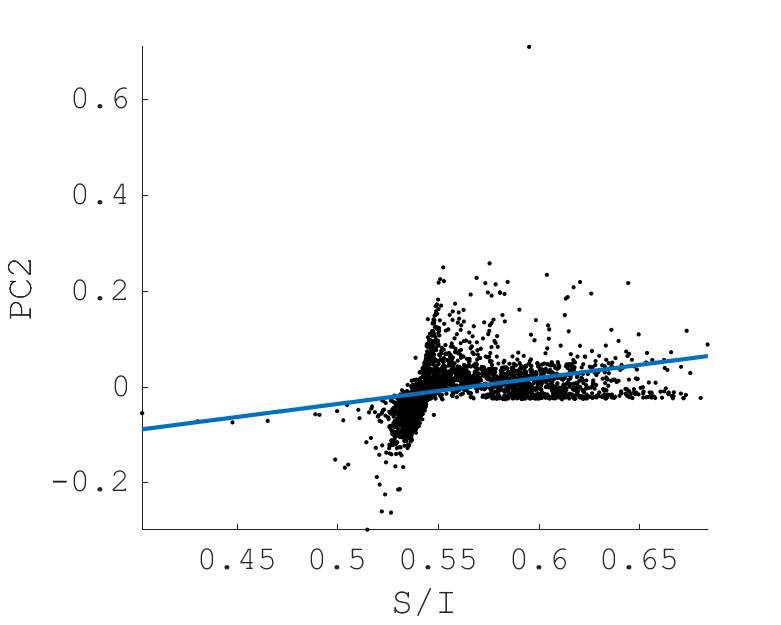
\includegraphics[max width=\textwidth]{figs/comp/melcomp_3/21.png}
 \caption{\hl{Caption}}
 \label{fig:S/I-PC2}
\end{figure} 




